\section{Methodology}
\label{sec:methods}


\begin{figure*}
    \centering
    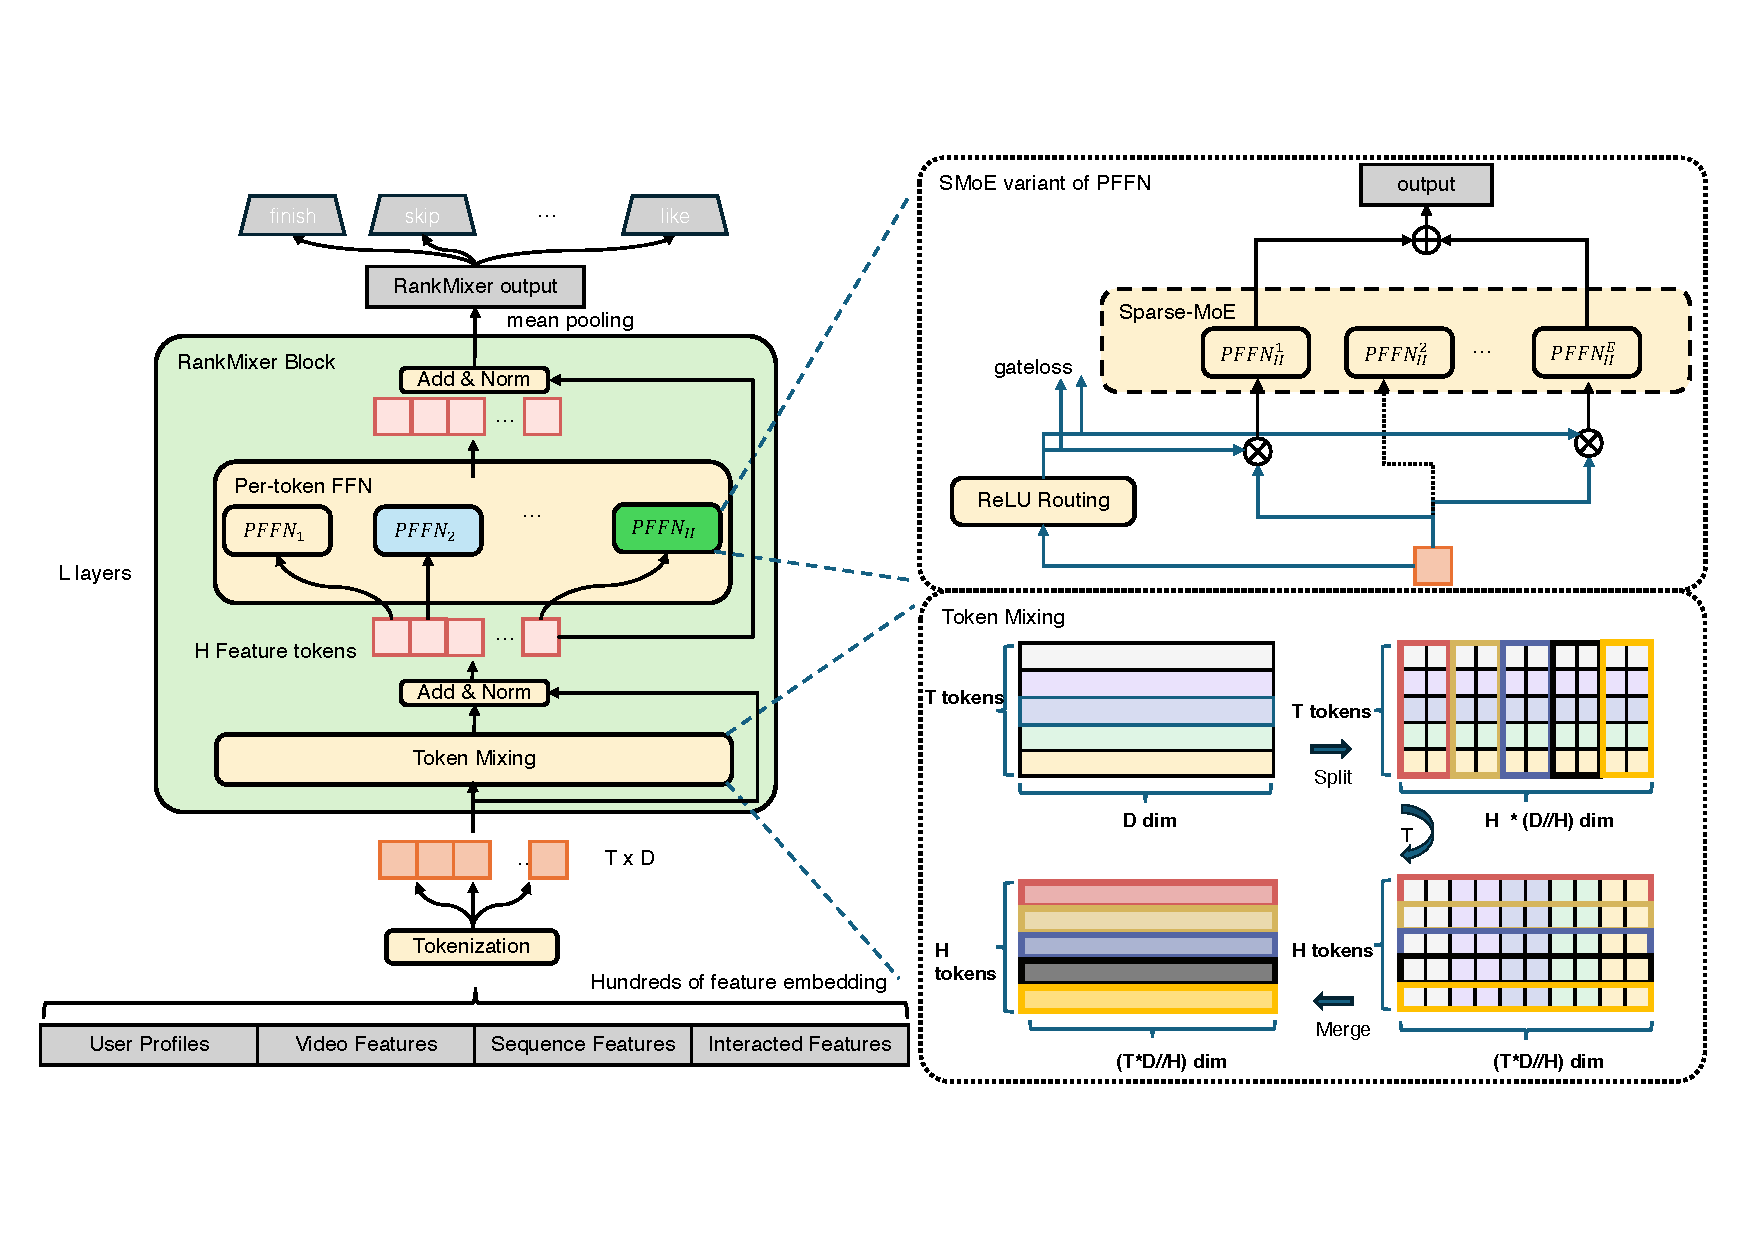
\includegraphics[width=0.85\linewidth]{img/RankMixer_arch_v3.pdf}
    \caption{The architecture of a RankMixer block. A RankMixer block consists of two modules: \textbf{Multi-head Token Mixing} and \textbf{SMoE based Per-token FFN}. The token-mixing module divides each token’s embedding into $H$ smaller parts (heads), then recombines these parts across tokens to create new mixed tokens. This allows information from different features to interact with each other.}
    \label{fig:arch_overall}
\end{figure*}

% \begin{figure}
%     \centering
%     \includegraphics[width=0.8\linewidth]{img/RankMixer_overview_v2.pdf}
%     \caption{The overall architecture of RankMixer. First the input $\mathbf{e}_{\text{input}}$ is split into tokens. Each token encodes a group of feature embeddings with high semantic similarity. Then, $N$ RankMixer blocks are stacked to model feature interactions. The output of RankMixer $\mathbf{e}_{\text{output}}$ is the mean pooling of the output of the last RankMixer block.}
%     \label{fig:arch_overall}
% \end{figure}


 \subsection{Overall Architecture}
    RankMixer’s overall architecture consists of T input tokens processed by L successive RankMixer blocks, followed by an output pooling operator. Each RankMixer block has two main components: (1) a Multi-Head Token Mixing layer, and (2) a Per-Token Feed-Forward Network (PFFN) layer, as illustrated in Figure~\ref{fig:arch_overall} . 
    First, the input vector $\mathbf{e}_{\text{input}}$ is tokenized into $T$ feature tokens $\mathbf{x}_1, \mathbf{x}_2, ..., \mathbf{x}_T$, each representing a coherent feature vector.
    % we split the input $\mathbf{e}_{input}$ into $T$ tokens $\mathbf{x}_1, \mathbf{x}_2, ..., \mathbf{x}_T$ of the same dimension $D_{RankMixer}$. Each token encodes a group of feature embeddings with high semantic similarity. 
    RankMixer blocks iteratively refine token representations for $L$ layers through:
    % , the $n$-th RankMixer block is formulated as
    \begin{equation}
    \begin{split}
        \mathbf{S}_{n-1} &= {\rm LN}\left({\rm TokenMixing} \left( \mathbf{X}_{n-1} \right) +  \mathbf{X}_{n-1}\right),\\
         \mathbf{X}_{n} &= {\rm LN} \left({\rm PFFN} \left( \mathbf{S}_{n-1} \right)  +\mathbf{S}_{n-1} \right),
    \end{split}
    \end{equation}
    where ${\rm LN}(\cdot)$ is a layer normalization function, ${\rm TokenMixing}(\cdot)$ and ${\rm PFFN}(\cdot)$ are the multi-head Token Mixing module and the per-token FFN module, $\mathbf{X}_{n} \in \mathbb{R}^{T \times D}$ is the output of the $n$-th RankMixer block, $\mathbf{X}_{0} \in \mathbb{R}^{T \times D}$ is stacked by $\mathbf{x}_1, \mathbf{x}_2, ..., \mathbf{x}_T$, and $D$ is the hidden dimension of the model. 
    The output representation $\mathbf{o}_{\text{output}}$ derives from the mean pooling of final layers's representations $\mathbf{X}_{L}$ which will be used to compute the different task's predictions.  

\subsection{Input Layer and Feature Tokenization}

The first thing to build a large-scale recommendation model is to prepare inputs with abundant information, such as \textbf{User features} include user ID and other user information, \textbf{candidate features} include video ID, author ID etc., \textbf{Sequence Features}  processed through Sequence Module \cite{din,longer} to capture temporal interests, yielding $\mathbf{e}_s$ and \textbf{Cross Features}. the cross features between the user and the candidate. All the features will be transformed into embeddings with diverse dimensions.  

To enable efficient parallel computation in later stages, embeddings of varying dimensions must be transformed into dimension-aligned vectors, called feature-tokens. We refer to this embedding alignment process as tokenization. The simplest strategy is assigning one embedding per feature which introduces several challenges given typically hundreds of features. Having hundreds of tokens inevitably reduces the parameters and computation allocated per token to small fragments, resulting in insufficient modeling of important features and under-utilization of GPU cores. Conversely, too few tokens (e.g. a single token) degrade the model structure into a simple Deep Neural Network (DNN), unable to distinctly represent diverse feature spaces, which risks dominant features overshadowing others.

To overcome these issues, we propose a semantic-based tokenization approach with domain knowledge and group features into several semantically coherent clusters. These grouped features are sequentially concatenated into one embedding vector $e_{\text{input}} \;=\; [\,e_{1}; e_{2}; \dots; e_{N}\,]$, and subsequently partitioned into an appropriate number of tokens with fixed dimension sizes. Each feature token $x_i \in \mathbb{R}^{D}$ captures a set of feature embeddings that represent a similar semantic aspect. 
\begin{equation}
  \newline
  \text{x}_{i} \;=\; {\rm Proj}(e_{\text{input}}\bigl[d\cdot(i-1) : d\cdot i\bigr]),
  \quad i = 1,\dots,T,
  \label{eq:tokenization}
\end{equation}
where \(e_{\text{input}}\) is the concatenated embedding vector,
\(d\) is the fixed dimension per token, \(N\) is the number of
feature-groups, and \(T\) is the resulting token count and the ${\rm Proj}$ function maps the splitted embedding into $D$ dimension.
    % For each embedding $\mathbf{e}_t$, we apply a two-layer MLP architecture to enable group-wise feature interaction and dimensional alignment:
    % \begin{equation}
    %     \mathbf{x}_t = {\rm Proj}(\mathbf{e_t}),
    % \end{equation}
    % where
    % \begin{equation}
    %     {\rm Proj}(\mathbf{e_t}) = f_{\text{proj}}^{t,2} \left({\rm Gelu} \left(f_{\text{proj}}^{t,1} \left(\mathbf{e}_t \right) \right) \right),
    % \end{equation}
    % and
    % \begin{equation}
    %     f_{\text{proj}}^{t,i}(\mathbf{x})=\mathbf{x}\mathbf{W}_{\text{proj}}^{t, i} + \mathbf{b}_{\text{proj}}^{t,i}
    % \end{equation}
    % is the $i$-th layer MLP architecture.
    % A Gelu activation function ~\cite{Gelu} ${\rm Gelu}(\cdot)$ is applied after the first MLP layer, and $\mathbf{x}_t \in \mathbb{R}^{D_{\text{RankMixer}}}$ is the $t$-th token, where $D_{\text{RankMixer}}$ is the token dimension.
    
    % We summarize the tokenization procedure as
    % \begin{equation}
    %     \mathbf{x}_1, \mathbf{x}_2, ..., \mathbf{x}_T = {\rm Tokenize} \left( \mathbf{e}_{\text{input}} \right),
    % \end{equation}
    % where
    % \begin{equation}
    %     {\rm Tokenize} \left( \mathbf{e}_{\text{input}} \right) = {\rm Proj} \left({\rm Split} \left( \mathbf{e}_{\text{input}} \right) \right).
    % \end{equation}  

% As the scale of the model increases, the input representation must evolve to retain its capacity to learn relevant patterns. A common approach is to increase the size of the embedding table, which imposes a heavy load on the parameter server, making the parameter server become a bottleneck in terms of memory and bandwidth. To further enrich the input representation, 
% we adopt 2-layer DHEN~\cite{zhang2022dhen} as a low-order feature interaction module for $\mathbf{e}_u$, $\mathbf{e}_v$ and $\mathbf{e}_s$ before RankMixer. We choose DCN~\cite{wang2021dcn} and self-attention~\cite{transformer} as the interaction modules in DHEN. Denote the output of DHEN as $\mathbf{e}_h$, and the input of RankMixer can be expressed as
% \begin{equation}
%     \mathbf{e}_{\text{input}} = {\rm Concat} \left( \mathbf{e}_u, \mathbf{e}_v, \mathbf{e}_s, \mathbf{e}_h \right),
% \end{equation}
% where $\mathbf{e}_{\text{input}} \in \mathbb{R}^{D_{\text{input}}}$ is a $D_{\text{input}}$ dimensional vector.
     
    
  \subsection{RankMixer Block}
    % We will introduce how to split $\mathbf{e}_{input}$ into tokens, the multi-head Token Mixing module and the per-token FFN module in the following parts.
    
  % \subsubsection{Tokenization}

  %   In large-scale industrial recommendation models, the input dimension $D_{\text{input}}$ is ofen very large, making direct application of deep MLPs to the input vector $\mathbf{e}_{\text{input}}$ computationally expensive and ineffective. 
  %   % Additionally, the model may struggle to learn meaningful feature interactions with such a large fully connected network.
  %   A common approach to address this problem is to split the input into tokens before applying feature interactions, such as DHEN~\cite{zhang2022dhen} and AutoInt~\cite{autoint}, where the number of tokens corresponds to the total number of features. However, this method can create critical limitations.
  %   Feature embeddings often exhibit varying dimensions due to their intrinsic information density, which poses two challenges. First, uniformly aligning embeddings to the maximum dimension results in excessive padding. Second, projecting all feature embeddings into the same dimension generates numerous small matrix operations, leading to under-utilization of GPU cores.

    
    
  \subsubsection{Multi-head Token Mixing}

    % After the inner-token feature interaction, we design the multi-head Token Mixing module to enable effective information exchange across tokens.
    To facilitate effective information exchange across tokens which is important for feature cross and global information modeling, we introduce the multi-head Token Mixing module.
    Each token is evenly divided into $H$ heads, with the $h$-th head of token $\mathbf{x}_t$ denoted as $x_t^h$:
    \begin{equation}
        \Bigl[\,
             \mathbf{x}_t^{(1)}
             \;\Vert\;
             \mathbf{x}_t^{(2)}
             \;\Vert\;\dots\;\Vert\;
             \mathbf{x}_t^{(H)}
            \Bigr] = {\rm SplitHead} \left( \mathbf{x}_t \right). 
    \end{equation}
    These heads can be seen as projections of the token $\mathbf{x}_t$ into a lower-dimensional feature subspace since recommendation is task taking different perspectives into considerations.
    % $x_t^h$ can be considered as a projection from the token $t$ into a subspace:
    Token Mixing is used to fuse these sub-space vector for global feature interactions. Formally, the $h$-th token $\mathbf{s}^{h}$ corresponding to the $h$-th head after the multi-head Token Mixing is constructed as:
    \begin{equation}
        \mathbf{s}^{h} = {\rm Concat}\left( \mathbf{x}_1^{h}, \mathbf{x}_2^{h}, ..., \mathbf{x}_T^{h} \right).
    \end{equation}
    The output of the multi-head Token Mixing module is $\mathbf{S} \in \mathbb{R}^{H \times \frac{TD}{H}}$, which is stacked by all the shuffled tokens $\mathbf{s}_{1}, \mathbf{s}_{2}, ..., \mathbf{s}_{H}$. In this work, we set $H=T$ to maintain the same number of tokens after Token Mixing for residual connection.

    % We summarize the multi-head Token Mixing operation as follows:
    
    % \begin{equation}
    %     {\rm TokenMixing} \left( \mathbf{x}_1, \mathbf{x}_2, ..., \mathbf{x}_T \right) = {\rm Merge}\left( {\rm SplitHead} \left( \mathbf{x}_1, \mathbf{x}_2, ..., \mathbf{x}_T \right) \right).
    % \end{equation}
    
    After a residual connection and normalization module we can generate
    \begin{equation}
        \mathbf{s}_1, \mathbf{s}_2, ..., \mathbf{s}_T = {\rm LN}\left({\rm TokenMixing} \left( \mathbf{x}_1, \mathbf{x}_2, ..., \mathbf{x}_T \right) + \left( \mathbf{x}_1, \mathbf{x}_2, ..., \mathbf{x}_T \right)\right),
    \end{equation}
    
    Although self-attention has proven highly effective in large language models, we find it to be suboptimal for recommendation systems.
    % In recommendation tasks, the feature spaces are inherently heterogeneous, with user demographics, item attributes, and interaction contexts existing in distinct semantic and dimensional domains.
    % This contrasts sharply with NLP paradigms, where all tokens 
    In self-attention, attention weights are calculated using the inner product of tokens. 
    This method works well for NLP, where all tokens share a unified embedding space. 
    However, in recommendation tasks, the feature spaces are inherently heterogeneous.
    Computing an inner-product similarity between two heterogeneous semantic spaces is notoriously difficult—particularly in recommender systems, where the ID space of the features from user and item side may contain hundreds of millions of elements.
    Consequently, applying self-attention to such diverse inputs does not outperform the parameter-free multi-head Token Mixing approach and consumes more computations, Memory IO operations and GPU memory usage.
    
  \subsubsection{Per-token FFN}
    Previous DLRM and DHEN models tend to mix features from many disparate semantic spaces in a single interaction module, which may causes high-frequency fields dominate drowning out lower-frequency or long-tail signals and ultimately hurting overall recommendation quality.
    We introduce a parameter-isolated feed-forward network architecture, termed per-token FFN. In traditional designs, the parameters of FFN are shared across all tokens, but our approach processes each token with dedicated transformations, thus isolating the parameters for each token. For the $t$-th token $\mathbf{s}_t$, the per-token FFN can be expressed as
    \begin{equation}
        \mathbf{v}_t = f_{\text{pffn}}^{t,2} \left({\rm Gelu} \left(f_{\text{pffn}}^{t,1} \left(\mathbf{s}_t \right) \right) \right),
    \end{equation}
    where
    \begin{equation}
        f_{\text{pffn}}^{t,i}(\mathbf{x})=\mathbf{x}\mathbf{W}_{\text{pffn}}^{t, i} + \mathbf{b}_{\text{pffn}}^{t, i}
    \end{equation}
    % where $f_{pffn}^{t,i}(\cdot)$ 
    is the $i$-th layer MLP of the per-token FFN, 
    % $f_{pffn}^{t,i}(\mathbf{x})=\mathbf{x}\mathbf{W}_{pffn}^{t, i} + \mathbf{b}_{pffn}^{t, i}$, 
    $\mathbf{W}_{\text{pffn}}^{t, 1} \in \mathbb{R}^{D \times kD}$, 
    $\mathbf{b}_{\text{pffn}}^{t, 1} \in \mathbb{R}^{kD}$,
    $\mathbf{W}_{\text{pffn}}^{t, 2} \in \mathbb{R}^{kD \times D}$, 
    $\mathbf{b}_{\text{pffn}}^{t, 2} \in \mathbb{R}^{D}$,
    $k$ is a hyperparameter to adjust the hidden dimension of the per-token FFN,
    ${\rm Gelu(\cdot)}$ is the Gelu activation function, $\mathbf{s}_t \in \mathbb{R}^{D}$ is the $t$-th token.

    We summarize the Per-token FFN module as
    \begin{equation}
        \mathbf{v}_1, \mathbf{v}_2, ..., \mathbf{v}_T = {\rm PFFN}\left( \mathbf{s}_1, \mathbf{s}_2, ..., \mathbf{s}_T \right), 
    \end{equation}
    where
    \begin{equation}
        {\rm PFFN}\left( \mathbf{s}_1, \mathbf{s}_2, ..., \mathbf{s}_T \right) = f_{\text{pffn}}^{t,2} \left({\rm Gelu} \left(f_{\text{pffn}}^{t,1} \left(\mathbf{s}_1, \mathbf{s}_2, ..., \mathbf{s}_T \right) \right) \right).
    \end{equation}
Compared to the parameter-all-shared FFN, per-token FFN enhances the modeling ability by introducing more parameters while keeping the computational complexity unchanged.

It is worth emphasizing that a Per-token FFN differs from MMoE experts in that each Per-token FFN sees a distinct token input, whereas all experts in a MMoE share the same input.
Unlike a MMoE, where many experts process the same input, and unlike a Transformer, where different input share one FFN, RankMixer splits the inputs and the parameters simultaneously which is good for learning diversity in different feature sub-spaces.


% Building upon the success of feed-forward networks (FFNs) in Transformer \cite{transformer} and MLP-Mixer \cite{mlpmixer}, we introduce a **parameter-isolated FFN architecture** that prevents representation collapse in recommendation scenarios. While traditional designs share FFN parameters across tokens, our formulation processes each token \(\mathbf{t}_i \in \mathbb{R}^{d_{mixer}}\) with dedicated transformations:  

% \[
% \mathbf{t}'_i = \mathbf{W}_2^{(i)} \cdot \text{GELU}(\mathbf{W}_1^{(i)} \mathbf{t}_i + \mathbf{b}_1^{(i)}) + \mathbf{b}_2^{(i)}
% \]  
% where \(\mathbf{W}_1^{(i)}, \mathbf{W}_2^{(i)}\) are token-specific weight matrices. This contrasts with standard FFNs that enforce \(\mathbf{W}_1^{(i)} = \mathbf{W}_1, \mathbf{W}_2^{(i)} = \mathbf{W}_2\) for all \(i\).  

% **Motivation from Representation Collapse**: The mix-up module generates synthetic tokens with high inter-token similarity (Figure 5). Shared FFN parameters amplify this redundancy through identical nonlinear transformations, leading to token matrix rank degradation. Let \(\text{rank}(\mathbf{T})\) denote the rank of token matrix:  

% \[
% \text{rank}(\mathbf{T}') \leq \min(\text{rank}(\mathbf{T}), \text{rank}(\mathbf{W}_1\mathbf{W}_2))  
% \]  

% Shared weights impose a fixed-rank bottleneck (\(\text{rank}(\mathbf{W}_1\mathbf{W}_2) \approx 64\) in practice), collapsing token diversity. Our per-token design circumvents this by allowing each token to learn unique projection trajectories.  

% **Key Advantages**:  
% 1. **Diversity Preservation**: Each FFN head adds directional variance to the token manifold.  
% 2. **Hardware Efficiency**: Despite \(n\)-fold parameter growth, FLOPs remain unchanged as parallel computation leverages GPU tensor cores:  
%    \[
%    \text{FLOPs} = 2n \cdot d_{mixer} \cdot d_{ffn} = \text{Constant w.r.t. Sharing}
%    \]  
% 3. **Adaptive Feature Learning**: High-information tokens (e.g., user ID embeddings) automatically allocate larger weight norms (\(\|\mathbf{W}^{(i)}\|_F\)) through gradient-based training.  

% Experiments on industrial datasets demonstrate our design achieves **2.7% AUC lift** versus shared-FFN baselines under identical computational budgets (Table 4). Further analysis reveals:  
% - The token matrix rank increases from 64 (shared) to 218 (per-token)  
% - Top-5 singular values account for 89% energy in shared FFN vs. 62% in per-token  
% - Training convergence accelerates by 18% due to reduced gradient conflict  

% Ablation studies (Figure 6) show parameter isolation contributes 73% of total performance gains, outweighing mix-up (19%) and Auto-Split (8%). This validates per-token FFN as critical for maintaining representation power in large-scale recommendation systems.  

  


% \begin{figure}[b]
%     \centering
%     \includegraphics[width=0.9\linewidth]{img/training_arch.pdf}
%     \caption{Overall pipeline of model deployment }
%     \label{fig:training_arch}
% \end{figure}

 \subsection{Sparse MoE in RankMixer}
To further increase the scaling ROI, we can replace the dense FFNs of each pertoken  with
\emph{Sparse Mixture-of-Experts} (MoE) blocks, so that the model's capacity grows while computation cost
remains roughly constant.
Vanilla Sparse-MoE, however, degrades in RankMixer because:
(i) \textbf{uniform $k$-expert routing}.  Top-$k$ selection treats all feature tokens
equally, wasting the budget on low-information tokens and starving high-information ones, which hinders the model from capturing differences between tokens.
(ii) \textbf{expert under-training}.  Per-token FFNs already multiply parameters by
\#tokens; adding non-shared experts further explodes the expert count, producing
highly unbalanced routing and poorly trained experts;

We combine two complementary training strategies to solve the above problems.

%--------------------------- 1. ReLU-routed Sparse-MoE --------------------------------
\paragraph{ReLU Routing}
To grant tokens flexible expert counts and maintain differentiability, we replace the common
\(\text{Top}k {+} {\rm softmax} \) with a ReLU gate plus an adaptive $\ell_1$ penalty
\cite{Wang2024remoe}. Given the $j$-th expert $e_{i,j}(\cdot)$ for token $s_i\!\in\!\mathbb{R}^{d_h}$ and router $h(\cdot)$:
\begin{equation}
  G_{i, j} = {\rm ReLU} \bigl(h(\mathbf{s}_i)\bigr), \quad
  \mathbf{v}_i = \sum_{j=1}^{N_e} G_{i, j}\, e_{i, j}(\mathbf{s}_i),
  \label{eq:dsmoe_forward}
\end{equation}
where $N_e$ is the number of experts per token, $N_t$ is the number of tokens.
% \begin{equation}
%   R(x)= {\rm ReLU} (sW)\in\mathbb{R}^{E},
%   \label{eq:relu_gate}
% \end{equation}
% where $W\!\in\!\mathbb{R}^{d_h\times E}$.  
ReLU Routing will activate more experts for high-information tokens and improve the parameter efficiency.
Sparsity is steered by
\(\mathcal{L}_{\mathrm{reg}}\) with an coefficient~$\lambda$ that
keeps the average active-expert ratio near the budget:
\begin{equation}
  \mathcal{L}= \mathcal{L}_{\text{task}}
              +\lambda\,\mathcal{L}_{\mathrm{reg}},
  \quad
  \mathcal{L}_{\mathrm{reg}}
  =\sum_{i=1}^{N_t}\sum_{j=1}^{N_e} G_{i,j}.
  \label{eq:relu_loss}
\end{equation}

%-------------------------- 2. Dense-training / Sparse-inference -----------------------
\paragraph{Dense-training / Sparse-inference (DTSI-MoE)}

Inspired by \cite{pan2024ads}, two routers $h_{\text{train}}$ and $h_{\text{infer}}$ are adopted, and $\mathcal{L}_{\mathrm{reg}}$ is applied only to $h_{\text{infer}}$. Both $h_{\text{train}}$ and $h_{\text{infer}}$ are updated during training, while only $h_{\text{infer}}$ is used in inference. It turns out that DS-MoE makes experts do not suffer from under-training while reducing inference cost.

% \begin{equation}
%   \mathbf{v}_\text{sparse\_inference}
%   =\sum_{e:R(x)_e>0}R(x)_e\,e_e(\mathbf{s}).
%   \label{eq:relu_inf}
% \end{equation}

% For a token $s\!\in\!\mathbb{R}^{d_h}$, training router $h_{train}(\cdot)$, and experts $e_i(\cdot)$:
% \begin{equation}
%   G_i = {\rm ReLU} \bigl(h_{train}(s)\bigr), \quad
%   \mathbf{v}_\text{train} = \sum_{i=1}^{N} G_i\,e_i(\mathbf{s}).
%   \label{eq:dsmoe_forward}
% \end{equation}
% In inference we keep only a few experts using the following Dynamic Routing strategies.
% % \begin{equation}
% %   \mathbf{v}=\sum_{i\in\TopK(x)} G_i\,e_i(\mathbf{s}).
% %   \label{eq:sparse_inf}
% % \end{equation} 



 \subsection{Scaling Up Directions}
 RankMixer is intrinsically a highly parallel and extensible
architecture.  Its parameter count and computational cost can be
expanded along four orthogonal axes: Token count \textbf{\(T\)}, Model width \textbf{\(D\)}, Layers \textbf{\(L\)} and Expert Numbers \textbf{\(E\)}. 
For full-dense-activated version, parameter and forward FLOPs for one sample can be computed as
\begin{equation}
  \text{\#Param}_{}
  \;\approx\;
  2\,k\,L\,T\,D^{2},
  \qquad
  \text{FLOPs}_{}
  \;\approx\;
  4\,k\,L\,T\,D^{2},
  \label{eq:dense_cost}
\end{equation}
The $k$ is the scale ratio adjusting the hidden dimension of FFN.
In the \emph{Sparse-MoE} version, the \emph{effective} parameters and
compute per token are further scaled by the sparsity ratio~$s=\frac{\text{\#Activated\_Param}}{  \text{\#Total\_Param}}$.
%   \subsection{Engineering Optimization}

% Training large-scale models effectively for production deployment requires a distributed framework that balances computational efficiency, scalability, and robustness, as demonstrated in Figure~\ref{fig:training_arch}.

% In our framework, dense computations are performed on GPUs, while sparse computations are assigned to a configured parameter server (PS). This design leverages the characteristics of sparse and dense parameters: sparse parameters are trained asynchronously to accommodate high feature cardinality and mitigate the potential bottlenecks from frequent communication, while dense parameters are synchronized to ensure weight consistency across devices, thereby improving convergence reliability and stabilizing performance in complex models. Furthermore, a statistical threshold restricts low-frequency features from entering the model, preserving system efficiency and minimizing negative impacts on performance.

% Key engineering optimizations enhance both training and inference efficiency. BF16 precision is employed for embedding transmission and network-layer parameter computations, reducing memory and computational overhead without sacrificing model fidelity. For inference, the synchronization mechanism is refined to ensure second-level sparse updates and minute-level dense updates, achieving a balance between real-time responsiveness and scalable model updates. This design ensures that improvements to the dense model are propagated seamlessly to the online system.


    %\subsubsection{Offline Training}
      %\begin{itemize}
       % \item Training challenges encountered, handling gradient explosion, and how to reasonably clip.
       % \item Synchronous training framework.
      %\end{itemize}
    %\subsubsection{Online Serving}
      %\begin{itemize}
        %\item Challenges and optimizations after scaling.
      %\end{itemize}